% ADD THIS HEADER TO ALL NEW CHAPTER FILES FOR SUBFILES SUPPORT

% Allow independent compilation of this section for efficiency
\documentclass[../CLthesis.tex]{subfiles}

% Add the graphics path for subfiles support
\graphicspath{{\subfix{../images/}}}

% Optional for standalone compilation of this chapter.
% Remove these lines if the main thesis preamble already loads them.
\usepackage{tikz}
\usetikzlibrary{arrows.meta, positioning, shapes.geometric, calc}
\usepackage{pgfplots}
\pgfplotsset{compat=1.18}

% END OF SUBFILES HEADER

%%%%%%%%%%%%%%%%%%%%%%%%%%%%%%%%%%%%%%%%%%%%%%%%%%%%%%%%%%%%%%%%
% START OF DOCUMENT: Every chapter can be compiled separately
\begin{document}

\chapter{Datasets}%
\label{chap:material}

% Replace the citation keys below with the entries used in your bibliography.

\section{Overview}

This study constructs the dataset in two stages. The first stage builds a native corpus from real-world data sources. The second stage expands the low-resource Chinese and Japanese corpora through LLM-based augmentation. We adopt this two-stage design because anti-Christian hate speech is difficult to collect at sufficient scale in Chinese and Japanese through native retrieval alone. A purely keyword-based corpus would be too noisy, whereas a purely synthetic corpus would be insufficiently grounded in naturally occurring discourse. Our final design therefore combines native evidence, manual annotation, supervised filtering, and controlled augmentation.

The overall aim of dataset construction is not merely to collect texts that mention Christianity. Rather, this study seeks to construct an analytically useful corpus of \textit{anti-Christian hate expression}. In practice, this requires separating three related but distinct phenomena: general religious reference, Christianity-related discussion, and explicit hate speech. This distinction is particularly important in the present research setting, because keywords such as \textit{church}, \textit{Bible}, \textit{priest}, \textit{Jesus}, or their Chinese and Japanese counterparts often occur in neutral, journalistic, theological, or ironic contexts that should not be treated as hate speech.

To address this problem, the pipeline introduces multiple layers of control. First, candidate texts are retrieved by keyword from platform-specific sources or existing corpora. Second, manually annotated Chinese and Japanese datasets are created with two binary labels: topic relevance and hatefulness. Third, language-specific detectors are fine-tuned on these labeled sets and are then used to filter larger candidate pools. Finally, an English seed corpus is used to support LLM-based localization into Chinese and Japanese, with the generated texts again filtered by the fine-tuned classifiers. This layered procedure improves both topical precision and stylistic coverage.

Figure~\ref{fig:dataset-overall-pipeline} summarizes the full construction workflow.

\begin{figure}[htbp]
\centering
\resizebox{0.98\textwidth}{!}{
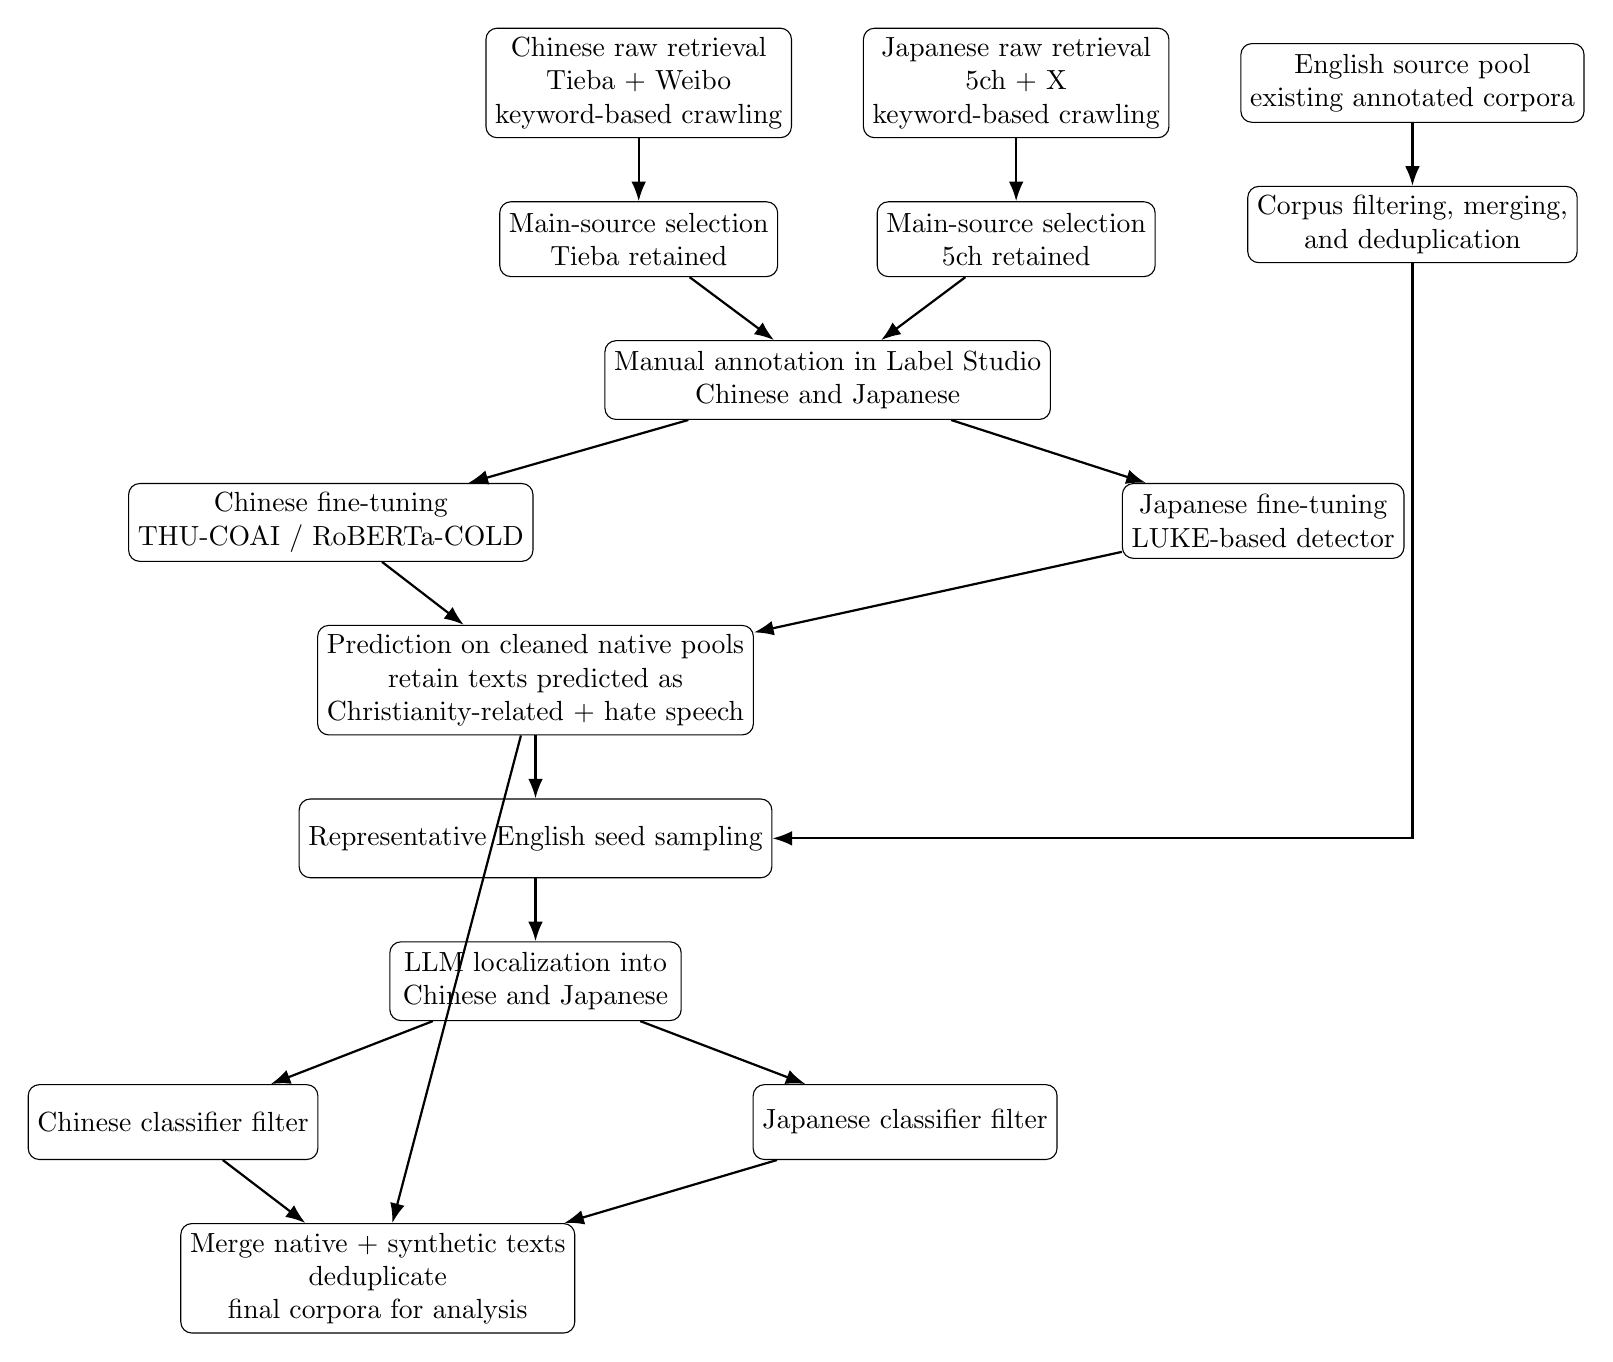
\begin{tikzpicture}[
node distance=8mm and 9mm,
box/.style={draw, rounded corners, align=center, minimum width=3.7cm, minimum height=1cm},
smallbox/.style={draw, rounded corners, align=center, minimum width=3.2cm, minimum height=0.95cm},
arrow/.style={-{Latex[length=2.5mm]}, thick}
]

\node[box] (zhraw) {Chinese raw retrieval\\Tieba + Weibo\\keyword-based crawling};
\node[box, right=of zhraw] (jaraw) {Japanese raw retrieval\\5ch + X\\keyword-based crawling};
\node[box, right=of jaraw] (enraw) {English source pool\\existing annotated corpora};

\node[smallbox, below=of zhraw] (zhmain) {Main-source selection\\Tieba retained};
\node[smallbox, below=of jaraw] (jamain) {Main-source selection\\5ch retained};
\node[smallbox, below=of enraw] (enmerge) {Corpus filtering, merging,\\and deduplication};

\node[box, below=of zhmain, xshift=2.4cm] (annot) {Manual annotation in Label Studio\\Chinese and Japanese};

\node[smallbox, below left=of annot] (zhft) {Chinese fine-tuning\\THU-COAI / RoBERTa-COLD};
\node[smallbox, below right=of annot] (jaft) {Japanese fine-tuning\\LUKE-based detector};

\node[box, below=of zhft, xshift=2.6cm] (nativefinal) {Prediction on cleaned native pools\\retain texts predicted as\\Christianity-related + hate speech};

\node[box, below=of nativefinal] (llmseed) {Representative English seed sampling};
\node[box, below=of llmseed] (llmgen) {LLM localization into\\Chinese and Japanese};
\node[smallbox, below left=of llmgen] (llmzh) {Chinese classifier filter};
\node[smallbox, below right=of llmgen] (llmja) {Japanese classifier filter};

\node[box, below=of llmzh, xshift=2.6cm] (mergefinal) {Merge native + synthetic texts\\deduplicate\\final corpora for analysis};

\draw[arrow] (zhraw) -- (zhmain);
\draw[arrow] (jaraw) -- (jamain);
\draw[arrow] (enraw) -- (enmerge);

\draw[arrow] (zhmain) -- (annot);
\draw[arrow] (jamain) -- (annot);

\draw[arrow] (annot) -- (zhft);
\draw[arrow] (annot) -- (jaft);

\draw[arrow] (zhft) -- (nativefinal);
\draw[arrow] (jaft) -- (nativefinal);

\draw[arrow] (enmerge) |- (llmseed);
\draw[arrow] (nativefinal) -- (llmseed);
\draw[arrow] (llmseed) -- (llmgen);
\draw[arrow] (llmgen) -- (llmzh);
\draw[arrow] (llmgen) -- (llmja);
\draw[arrow] (llmzh) -- (mergefinal);
\draw[arrow] (llmja) -- (mergefinal);
\draw[arrow] (nativefinal) -- (mergefinal);

\end{tikzpicture}
}
\caption{Overall dataset construction workflow adopted in this study. The final corpora are produced through a combination of native retrieval, manual annotation, supervised filtering, and controlled LLM-based augmentation.}
\label{fig:dataset-overall-pipeline}
\end{figure}

\section{Design Principles}

The construction procedure follows four principles.

First, we prioritize analytical precision over raw volume. Keyword-based retrieval is useful for obtaining candidate texts, but it is not sufficient for building the final corpus because many matched texts are neutral or only loosely relevant to the target.

Second, we distinguish between \textit{Christianity-related discourse} and \textit{anti-Christian hate speech}. This distinction is central to the annotation design and to the later supervised filtering stage.

Third, we treat native and synthetic data differently. Native texts provide naturally occurring discourse patterns from real platforms or existing corpora. Synthetic texts are used only as controlled supplements, not as replacements for native discourse.

Fourth, the final dataset is designed for downstream substantive analysis, including topic modeling and clustering, rather than for benchmark classification alone. For this reason, stylistic diversity and topical relevance are both treated as important construction goals.

\section{Native Chinese Data Construction}

\subsection{Retrieval and Source Selection}

The Chinese native pipeline began with keyword-based crawling from Tieba and Weibo. The keyword list included both neutral Christianity-related terms and derogatory or conflict-oriented expressions associated with anti-Christian discussion. This broad retrieval strategy was necessary because a narrow vocabulary would miss indirect hostility, sarcastic attacks, and pseudo-rational criticism, whereas an exclusively abusive keyword list would over-restrict the corpus to only the most explicit insults.

After initial collection and inspection, Weibo was not retained as the main Chinese source because it contributed too few usable texts for the purposes of this study. Tieba therefore became the main platform in the Chinese native pipeline. This choice was primarily empirical: the retained source was the one that provided sufficient candidate volume for later annotation and supervised filtering.

In the current repository snapshot, the raw Chinese candidate pool contains 78{,}874 texts, while the cleaned Chinese working pool contains 15{,}181 texts. The reduction in size reflects the removal of duplicates, trivial matches, empty items, and obviously irrelevant content. This sharp decrease also indicates the limits of keyword-based retrieval for the present task: large numbers of texts can mention Christian vocabulary without constituting anti-Christian hate speech.

\subsection{Manual Annotation}

Chinese annotation was conducted in Label Studio \citep{labelstudio}. We manually annotated 4{,}000 Chinese texts. Each item received two binary labels:

\begin{itemize}
\item \texttt{christianity\_related}: whether the text is substantively related to Christianity;
\item \texttt{hate\_speech}: whether the text expresses hate directed at the Christian target.
\end{itemize}

This two-step labeling design was adopted because many keyword-matched Chinese texts refer to Christianity without targeting Christians as a group. For example, some posts discuss the Vatican, Biblical narratives, church scandals, or religious institutions in descriptive or ironic terms without containing target-directed hate. A single-label design would obscure this difference.

The final Chinese annotated set contains 613 texts labeled as Christianity-related and 152 texts labeled as hate speech. These proportions show that explicit anti-Christian hate remains relatively rare even inside a curated candidate pool. This confirms that manual annotation is indispensable for defining the task boundary.

\subsection{Model Fine-Tuning and Native Final Set}

After annotation, this study fine-tuned a Chinese detector based on THU-COAI RoBERTa-COLD \citep{thucoai-roberta-cold}. The fine-tuned model was then applied to the cleaned Chinese candidate pool. We retained only texts predicted as both Christianity-related and hateful. In this way, the final native Chinese set was not created by simply collecting all keyword-matched items, but by passing the broader candidate pool through a task-specific supervised filter.

This stage produced 1{,}070 native Chinese hate texts. Although this is much smaller than the original retrieval pool, it is substantially more precise and better aligned with the analytical objective of the study.

\section{Native Japanese Data Construction}

\subsection{Retrieval and Source Selection}

The Japanese native pipeline followed the same general logic. Candidate texts were first collected from 5ch and X through keyword-based retrieval. The keyword list combined neutral Christian terminology with mocking, hostile, and conspiratorial expressions associated with anti-Christian discourse in Japanese online contexts.

In practice, X could not serve as the main Japanese source because its free access quota was too limited to support a sufficiently large working pool. The Japanese native dataset therefore relies primarily on 5ch. This decision was again pragmatic: the study retained the source that yielded enough retrievable material for annotation and later supervised selection.

In the current repository snapshot, the raw Japanese candidate pool contains 43{,}101 texts, whereas the cleaned Japanese working pool contains 4{,}181 texts. As in Chinese, this large reduction shows that keyword-based retrieval alone captures many texts that are topically adjacent but not analytically suitable for the target task.

\subsection{Manual Annotation}

Japanese annotation was also conducted in Label Studio \citep{labelstudio}. We manually annotated 4{,}084 Japanese texts. The same two binary labels were used:

\begin{itemize}
\item \texttt{christianity\_related};
\item \texttt{hate\_speech}.
\end{itemize}

Using the same annotation scheme across Chinese and Japanese improves comparability between the two low-resource language settings. It also ensures that the later filtering stage is grounded in parallel operational definitions rather than language-specific label systems.

The final Japanese annotated set contains 690 Christianity-related texts and 102 hate-speech texts. The hate label is thus even rarer in Japanese than in Chinese, which further illustrates the scarcity of explicit anti-Christian hate in the raw Japanese candidate pool.

\subsection{Model Fine-Tuning and Native Final Set}

After annotation, this study fine-tuned a Japanese detector based on LUKE \citep{luke-japanese}. The fine-tuned Japanese classifier was then applied to the cleaned Japanese candidate pool. As in the Chinese pipeline, only texts predicted as both Christianity-related and hateful were retained.

This step yielded 1{,}445 native Japanese hate texts. The resulting corpus is therefore a post-filtered analytical set rather than a direct extraction of all crawled content.

Figure~\ref{fig:zh-ja-native-pipelines} presents the Chinese and Japanese native pipelines in parallel.

\begin{figure}[htbp]
\centering
\resizebox{0.98\textwidth}{!}{
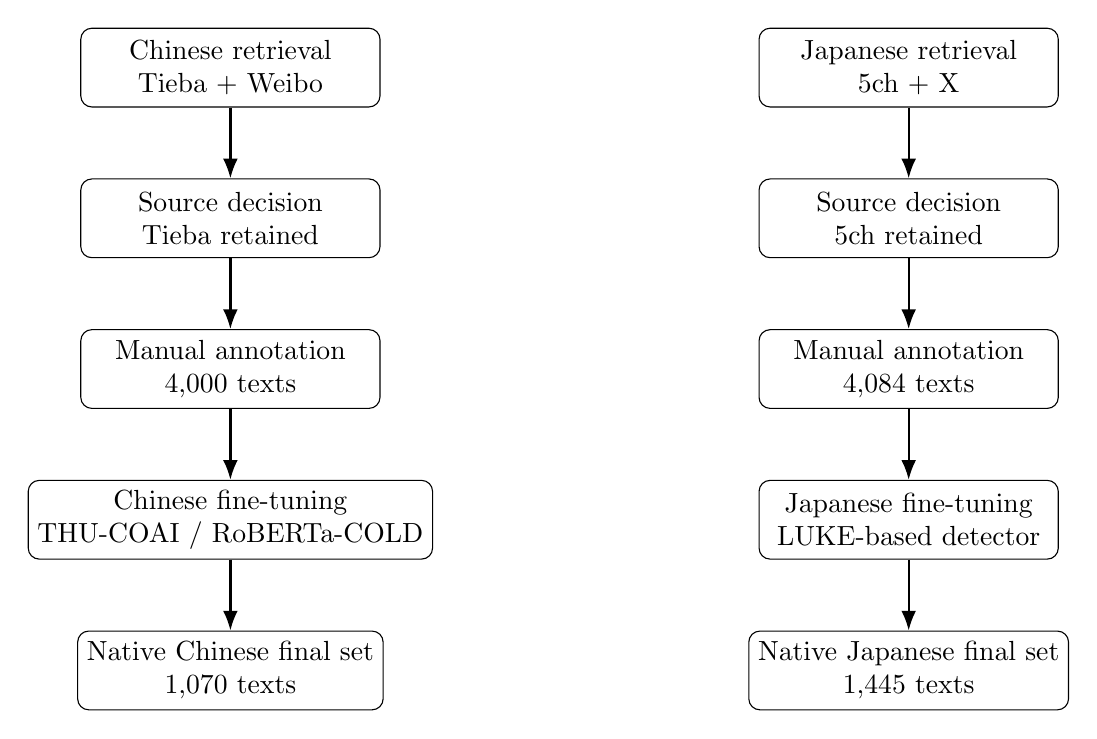
\begin{tikzpicture}[
node distance=9mm and 14mm,
box/.style={draw, rounded corners, align=center, minimum width=3.8cm, minimum height=1cm},
arrow/.style={-{Latex[length=2.5mm]}, thick}
]

\node[box] (zh1) {Chinese retrieval\\Tieba + Weibo};
\node[box, below=of zh1] (zh2) {Source decision\\Tieba retained};
\node[box, below=of zh2] (zh3) {Manual annotation\\4{,}000 texts};
\node[box, below=of zh3] (zh4) {Chinese fine-tuning\\THU-COAI / RoBERTa-COLD};
\node[box, below=of zh4] (zh5) {Native Chinese final set\\1{,}070 texts};

\node[box, right=4.8cm of zh1] (ja1) {Japanese retrieval\\5ch + X};
\node[box, below=of ja1] (ja2) {Source decision\\5ch retained};
\node[box, below=of ja2] (ja3) {Manual annotation\\4{,}084 texts};
\node[box, below=of ja3] (ja4) {Japanese fine-tuning\\LUKE-based detector};
\node[box, below=of ja4] (ja5) {Native Japanese final set\\1{,}445 texts};

\draw[arrow] (zh1) -- (zh2);
\draw[arrow] (zh2) -- (zh3);
\draw[arrow] (zh3) -- (zh4);
\draw[arrow] (zh4) -- (zh5);

\draw[arrow] (ja1) -- (ja2);
\draw[arrow] (ja2) -- (ja3);
\draw[arrow] (ja3) -- (ja4);
\draw[arrow] (ja4) -- (ja5);

\end{tikzpicture}
}
\caption{Parallel native-data construction pipelines for Chinese and Japanese. In both languages, two platforms were initially considered, but the final native corpus was built around the source that offered sufficient usable material for annotation and filtering.}
\label{fig:zh-ja-native-pipelines}
\end{figure}

\section{English Data from Existing Annotated Corpora}

The English corpus follows a different construction logic. Rather than building a new crawling pipeline, this study reuses and merges several existing annotated resources that contain Christian-target or religion-related labels, including HateXplain, Jigsaw, MLMA, and Measuring Hate Speech \citep{mathew_hatexplain_2021, jigsaw-unintended-bias, mlma, measuring-hate-speech}. Each source was filtered to retain Christian-target examples, after which the filtered files were merged and deduplicated.

This design offers two advantages. First, English already has richer publicly available resources for identity-based hate speech than Chinese and Japanese. Second, the English pool provides a broader range of attack patterns, lexical styles, and discourse settings than could be collected efficiently through a small independent crawl. Accordingly, the English corpus serves not only as the English-language dataset in the overall design, but also as the seed reservoir for later cross-lingual augmentation.

The merged English file in the current repository contains 58{,}940 texts. Its source composition is shown in Table~\ref{tab:english-sources}. Most items come from Jigsaw, while the other corpora contribute smaller but still valuable Christian-target subsets.

\begin{table}[htbp]
\centering
\small
\begin{tabular}{lr}
\hline
Source corpus & Number of texts \\
\hline
Jigsaw & 55{,}984 \\
Measuring Hate Speech & 2{,}744 \\
HateXplain & 208 \\
MLMA & 4 \\
\hline
Total & 58{,}940 \\
\hline
\end{tabular}
\caption{Composition of the merged English corpus after Christian-target filtering and deduplication.}
\label{tab:english-sources}
\end{table}

Unlike the Chinese and Japanese native datasets, the English corpus was not newly annotated in this study. Its role lies in target-specific filtering, merging, and later reuse for augmentation.

\section{Annotation Logic and Sampling Strategy}

The annotation stage is the central mechanism through which noisy candidate retrieval is converted into a task-defined corpus. Importantly, annotation in this study is not based on a simple one-step hate versus non-hate decision. Instead, the procedure first asks whether a text is substantially related to Christianity and only then asks whether it contains hate speech. This sequential logic is shown in Figure~\ref{fig:annotation-logic}.

\begin{figure}[htbp]
\centering
\resizebox{0.82\textwidth}{!}{
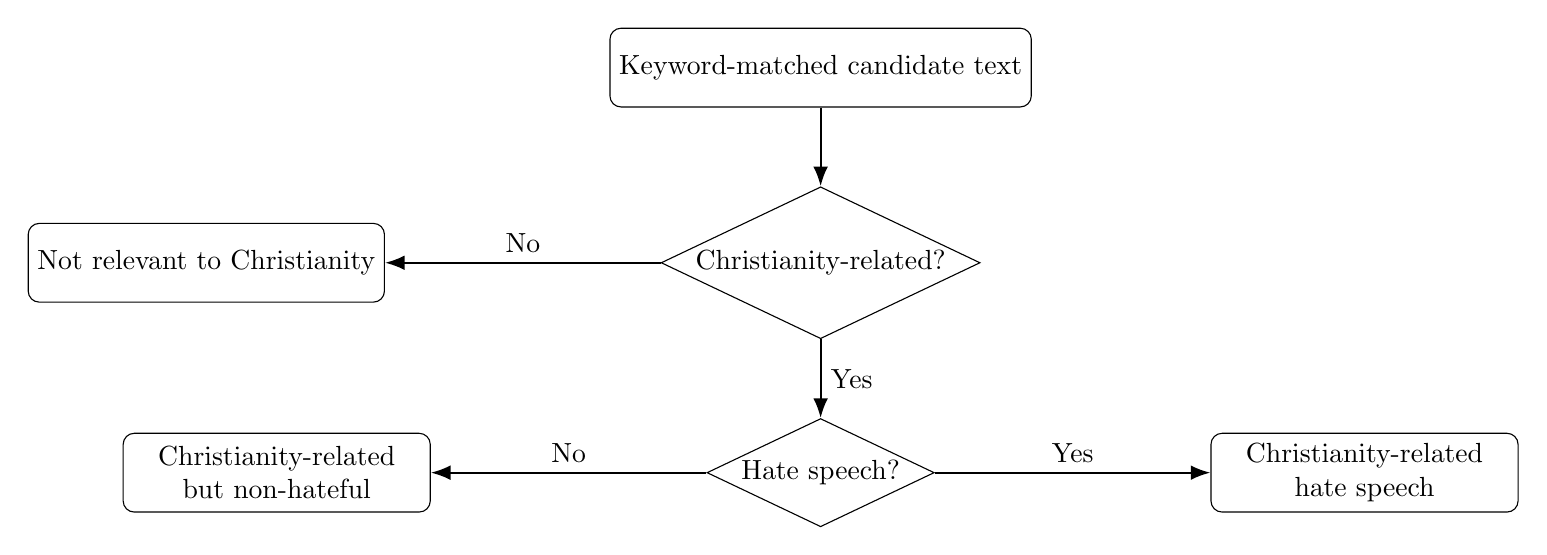
\begin{tikzpicture}[
node distance=10mm and 14mm,
box/.style={draw, rounded corners, align=center, minimum width=3.9cm, minimum height=1cm},
decision/.style={diamond, draw, align=center, aspect=2.1, inner sep=1pt},
arrow/.style={-{Latex[length=2.5mm]}, thick}
]

\node[box] (cand) {Keyword-matched candidate text};
\node[decision, below=of cand] (rel) {Christianity-related?};
\node[decision, below=of rel] (hate) {Hate speech?};

\node[box, left=3.5cm of rel] (nonrel) {Not relevant to Christianity};
\node[box, left=3.5cm of hate] (relatednonhate) {Christianity-related\\but non-hateful};
\node[box, right=3.5cm of hate] (target) {Christianity-related\\hate speech};

\draw[arrow] (cand) -- (rel);
\draw[arrow] (rel) -- node[right] {Yes} (hate);
\draw[arrow] (rel) -- node[above] {No} (nonrel);
\draw[arrow] (hate) -- node[above] {No} (relatednonhate);
\draw[arrow] (hate) -- node[above] {Yes} (target);

\end{tikzpicture}
}
\caption{Sequential annotation logic used in this study. A text must first be judged as Christianity-related before it can be classified as anti-Christian hate speech.}
\label{fig:annotation-logic}
\end{figure}

This annotation design is especially important for the religious domain. Posts discussing churches, clergy, scripture, or religious institutions may be critical, ironic, or controversial without being target-directed hate speech. By separating topic relevance from hatefulness, the present study reduces false positives and creates a more stable basis for model fine-tuning.

Annotation efficiency was also improved through uncertainty-oriented sampling. Instead of relying on simple random sampling alone, the pre-annotation pipeline over-sampled borderline cases, including texts with model disagreement or low confidence. This design directs manual effort toward examples that are most informative for clarifying the decision boundary. A smaller number of high-confidence positive and high-confidence negative examples were then added to maintain class coverage.

\section{Why LLM Augmentation Was Needed}

Although the native Chinese and Japanese pipelines produced usable corpora, the resulting native hate sets remained limited in size. More importantly, they also reflected the structural limits of platform availability. Chinese native data were concentrated in Tieba, and Japanese native data were concentrated in 5ch. In both languages, explicit anti-Christian hate was rare even after careful retrieval. For this reason, augmentation was necessary to improve stylistic and thematic coverage.

However, this study did not adopt synthetic augmentation uncritically. The first design considered direct few-shot generation in Chinese and Japanese. In that version, the LLM was prompted to generate new texts directly from small sets of example sentences. After evaluation, this approach was not retained in the final pipeline because the outputs were overly repetitive. They tended to recycle the same rhetorical structure, attack frame, and emotional tone, which would have narrowed rather than broadened the discourse space of the final corpus.

The final augmentation strategy therefore shifted from \textit{direct few-shot generation} to \textit{seed-based localization}. This change is methodologically important. Rather than asking the LLM to invent hostile texts from scratch, we anchored generation in representative English texts drawn from a large existing corpus. The synthetic Chinese and Japanese texts were then generated as culturally localized re-expressions of those English seed texts.

\section{LLM-Augmented Chinese and Japanese Data}

\subsection{Seed-Based Localization}

The final augmentation pipeline begins with representative English seed sampling from the merged English corpus. The purpose of this step is not to maximize frequency, but to preserve diversity across attack styles, themes, and rhetorical forms. The selected English texts are then given to the LLM as source material for localized Chinese and Japanese generation.

The prompts explicitly ask for cultural alignment rather than literal translation. The model is instructed to preserve the underlying attack logic while rewriting the expression in a form that resembles local online discourse. For Chinese, the intended style is closer to hostile expression on Chinese social platforms. For Japanese, the intended style is closer to forum-style or X-style antagonistic discourse. This approach aims to transfer semantic patterns while adapting lexical and stylistic realization \citep{cross-lingual-llm-localization, llm-style-transfer}.

\subsection{Post-Generation Filtering}

The generated outputs are not accepted automatically. Instead, the localized Chinese and Japanese texts are passed through the corresponding fine-tuned classifiers. Only texts predicted as both Christianity-related and hateful are retained. This post-generation filtering serves two purposes. First, it removes synthetic outputs that drift away from the topic or lose the hate component. Second, it ensures that native and synthetic texts satisfy the same operational task definition.

After filtering, the augmentation stage yields 895 Chinese synthetic texts and 915 Japanese synthetic texts. These are then merged with the native Chinese and Japanese sets and deduplicated to produce the final mixed corpora.

Figure~\ref{fig:llm-augmentation-pipeline} illustrates the final augmentation workflow.

\begin{figure}[htbp]
\centering
\resizebox{0.98\textwidth}{!}{
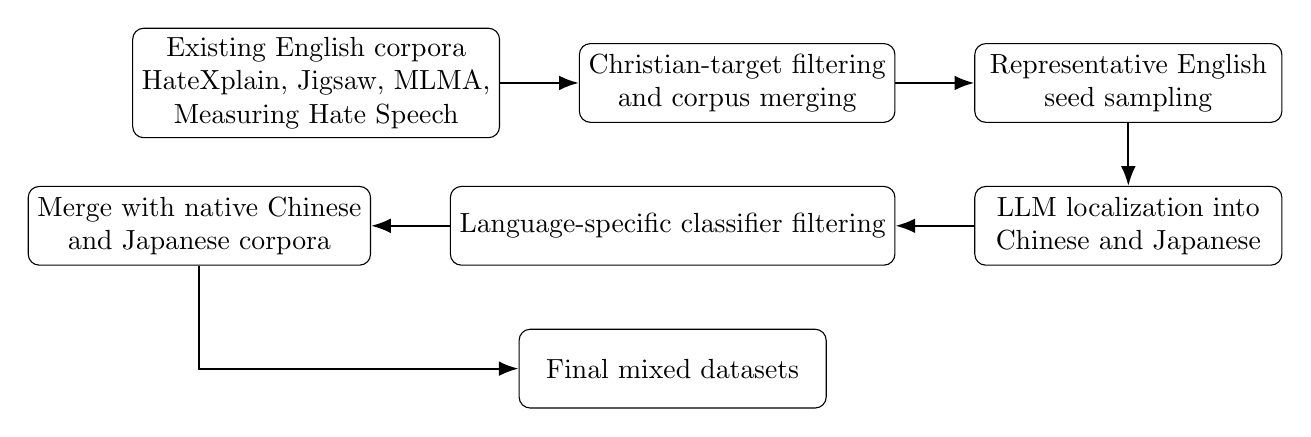
\begin{tikzpicture}[
node distance=8mm and 10mm,
box/.style={draw, rounded corners, align=center, minimum width=3.9cm, minimum height=1cm},
arrow/.style={-{Latex[length=2.5mm]}, thick}
]

\node[box] (eng1) {Existing English corpora\\HateXplain, Jigsaw, MLMA,\\Measuring Hate Speech};
\node[box, right=of eng1] (eng2) {Christian-target filtering\\and corpus merging};
\node[box, right=of eng2] (eng3) {Representative English\\seed sampling};
\node[box, below=of eng3] (llm1) {LLM localization into\\Chinese and Japanese};
\node[box, left=of llm1] (llm2) {Language-specific classifier filtering};
\node[box, left=of llm2] (llm3) {Merge with native Chinese\\and Japanese corpora};
\node[box, below=of llm2] (llm4) {Final mixed datasets};

\draw[arrow] (eng1) -- (eng2);
\draw[arrow] (eng2) -- (eng3);
\draw[arrow] (eng3) -- (llm1);
\draw[arrow] (llm1) -- (llm2);
\draw[arrow] (llm2) -- (llm3);
\draw[arrow] (llm3) |- (llm4);

\end{tikzpicture}
}
\caption{Final LLM-based augmentation pipeline used in this study. Instead of relying on direct few-shot generation alone, the retained design localizes representative English seed texts into Chinese and Japanese and then filters the outputs with fine-tuned classifiers.}
\label{fig:llm-augmentation-pipeline}
\end{figure}

\subsection{Role of Synthetic Data}

The synthetic portion of the final corpus should be interpreted as a controlled supplement rather than as a substitute for native discourse. Its role is to expand the available expression space in two low-resource languages, especially with respect to rhetorical variation and locally adapted attack forms. The synthetic data are therefore useful for enriching coverage, but they remain analytically distinct from naturally occurring platform texts. This distinction is important for later interpretation of clustering results and qualitative findings.

\section{Descriptive Statistics}

Table~\ref{tab:dataset-summary} presents the main dataset sizes across construction stages.

\begin{table}[htbp]
\centering
\small
\begin{tabular}{lrrrrrr}
\hline
Language & Raw Pool & Cleaned Pool & Manual Labels & Native Final & LLM Final & Mixed Final \\
\hline
Chinese  & 78{,}874 & 15{,}181 & 4{,}000 & 1{,}070 & 895 & 1{,}965 \\
Japanese & 43{,}101 & 4{,}181  & 4{,}084 & 1{,}445 & 915 & 2{,}360 \\
English  & --       & 58{,}940 & --      & 58{,}940 & --  & 58{,}940 \\
\hline
\end{tabular}
\caption{Dataset sizes across the main construction stages. English is built from existing annotated corpora rather than from a new platform-crawling pipeline.}
\label{tab:dataset-summary}
\end{table}

For the manually annotated Chinese and Japanese sets, the label distributions are summarized in Table~\ref{tab:annotation-distribution}. The figures illustrate the core challenge of the task: even after retrieval and candidate filtering, explicit anti-Christian hate remains a minority class.

\begin{table}[htbp]
\centering
\small
\begin{tabular}{lrrrr}
\hline
Language & Total annotated & Christianity-related & Hate speech & Hate ratio \\
\hline
Chinese  & 4{,}000 & 613 & 152 & 3.8\% \\
Japanese & 4{,}084 & 690 & 102 & 2.5\% \\
\hline
\end{tabular}
\caption{Label distribution in the manually annotated Chinese and Japanese datasets.}
\label{tab:annotation-distribution}
\end{table}

Figure~\ref{fig:dataset-size-comparison} compares the sizes of the native, synthetic, and final mixed datasets. The figure makes clear that Chinese and Japanese depend on both native and augmented data, whereas the English corpus is much larger and is not augmented in the same way.

\begin{figure}[htbp]
\centering
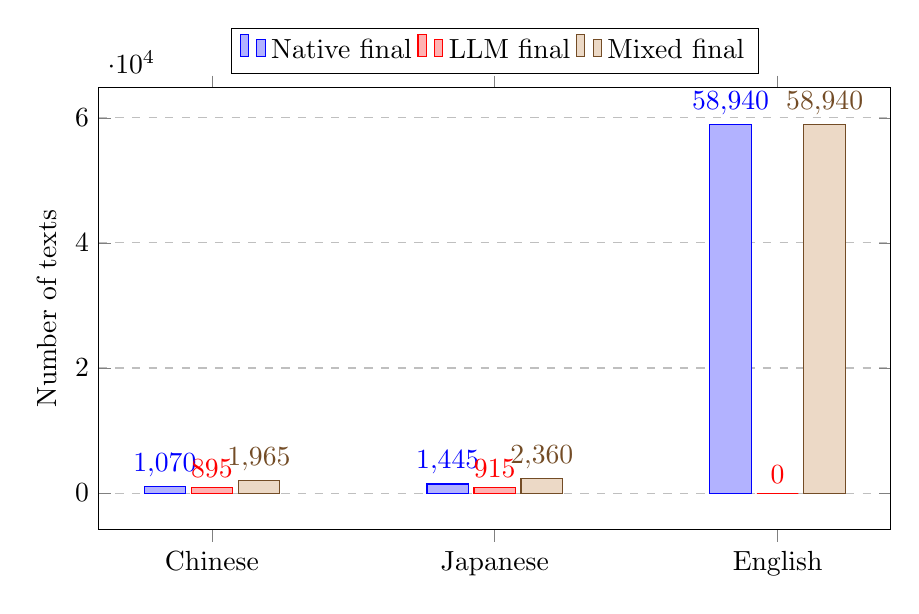
\begin{tikzpicture}
\begin{axis}[
ybar,
bar width=15pt,
width=0.96\textwidth,
height=7.2cm,
ylabel={Number of texts},
symbolic x coords={Chinese,Japanese,English},
xtick=data,
legend style={at={(0.5,1.03)}, anchor=south, legend columns=3},
ymajorgrids=true,
grid style=dashed,
nodes near coords,
nodes near coords align={vertical},
enlarge x limits=0.2
]
\addplot coordinates {(Chinese,1070) (Japanese,1445) (English,58940)};
\addplot coordinates {(Chinese,895) (Japanese,915) (English,0)};
\addplot coordinates {(Chinese,1965) (Japanese,2360) (English,58940)};
\legend{Native final, LLM final, Mixed final}
\end{axis}
\end{tikzpicture}
\caption{Size comparison of the final native, synthetic, and mixed datasets. Chinese and Japanese rely on both native and synthetic data, whereas the English dataset is constructed from existing annotated corpora and is not augmented in the same manner.}
\label{fig:dataset-size-comparison}
\end{figure}

\section{What Was Developed in This Study}

Several major components of the dataset construction process were developed directly in this study.

First, we built the Chinese and Japanese native pipelines, including keyword-based retrieval, cleaning, deduplication, and source selection. Second, we designed the two-label annotation scheme and manually annotated the core Chinese and Japanese datasets in Label Studio. Third, we fine-tuned language-specific detectors and used them to filter both native candidate pools and synthetic outputs. Fourth, we designed the final augmentation strategy in which representative English texts were localized into Chinese and Japanese and then filtered again before being admitted to the final corpora.

By contrast, the English portion of the data was not newly annotated in this study. Its contribution lies in Christian-target filtering, corpus integration, and later use as a cross-lingual support resource.

\section{Limitations}

The constructed datasets nonetheless retain several limitations.

First, the native Chinese and Japanese corpora remain platform-dependent. Because Tieba and 5ch were retained primarily on empirical grounds, the final corpora may reflect the discourse norms of those platforms more strongly than the wider online public sphere.

Second, keyword-based retrieval necessarily shapes the initial candidate space. Although later annotation and supervised filtering reduce this bias, some indirect or euphemistic forms of anti-Christian hostility that avoid overt religious vocabulary may remain underrepresented.

Third, the synthetic Chinese and Japanese texts are controlled supplements rather than naturally occurring discourse. Even after classifier filtering, they should not be interpreted as fully equivalent to native platform texts. Their primary value lies in expanding thematic and stylistic coverage under low-resource conditions.

Finally, the English corpus is much larger and structurally different from the Chinese and Japanese corpora. This asymmetry is one reason why English was used as the seed language for augmentation, but it also means that cross-lingual comparisons should be interpreted with caution.

\section{Chapter Summary}

This chapter has described the full dataset construction procedure used in this study. Chinese and Japanese native data were collected from platform-based retrieval, manually annotated with a two-step label design, and then filtered again with fine-tuned language-specific models. English data were built by filtering and merging several existing annotated corpora. On top of this native foundation, the study added controlled LLM-based augmentation by localizing representative English seed texts into Chinese and Japanese and filtering the results with the same operational criteria.

Taken together, this construction strategy offers a practical balance between empirical grounding and low-resource expansion. It keeps the final corpora anchored in real discourse while using controlled synthetic generation to improve stylistic and thematic coverage. For the analytical aims of this thesis, this balance is more valuable than either a small but purely native dataset or a large but weakly grounded synthetic one.

% self-defined macro: include bibliography even when compiling a single chapter
\subfilebibliography
\end{document}
